\section{Evaluation}
\label{res_overview}

\begin{table}[]
    \centering\small\footnotesize
    \caption{Evaluation results overview: Name, Side-channel Leaks\,(Leaks), 
        Secret-dependent Control-flows\,(CF), Secret-dependent Data-flows\,(DF),
        The number of instructions\,(\# Instructions), Symbolic Execution\,(SE) and Monte Carlo\,(MC) time.
    }\label{table:over_result}
    \vspace*{-5pt}
    \newlength{\x}
    \newlength{\y}
    \settowidth{\x}{~~}
    \settowidth{\y}{m}
    \addtolength{\x}{-1\y}
    \newcommand{\foo}{\mbox{\hspace*{\the\x}}}
%    \resizebox{1.9\columnwidth}{!}{
    \begin{threeparttable}
    \begin{tabular}{l@{}r@{~~}rrr@{~~}rr}
        \hline
        \textbf{Name}   & \textbf{\# Leaks} & \textbf{\# CF}         & \textbf{\# DF}
                           & \textbf{\# Instructions}    & \textbf{SE} & \textbf{MC}                                                    \\\hline
                                                 &                        &                     &                      &              & ms        & ms              \\\cline{6-7}
        AES\tnote{1}               & 68                     & 0                   & 68                   & 39,855        & 512     & 1,052         \\
        AES\tnote{2}                & 68                     & 0                   & 68                   & 39,855       & 520    & 1,057         \\
        AES\tnote{4}                & 75                     & 0                   & 75                   & 1,704        & 231    & 9,199        \\
        AES\tnote{5}                & 88                     & 0                   & 88                   & 1,350        & 36      & 1,924         \\
        AES\tnote{6}                & 88                     & 0                   & 88                   & 1,350        & 35      & 1,961        \\
        AES\tnote{7}                & 88                     & 0                   & 88                   & 1,420        & 36     & 2,161        \\
        AES\tnote{8}                & 88                     & 0                   & 88                   & 1,586        & 43      & 1,631        \\
        DES\tnote{1}                & 15                     & 0                   & 15                   & 4,596        & 58      & 162          \\
        DES\tnote{2}                & 15                     & 0                   & 15                   & 4,596        & 57      & 162           \\
        DES\tnote{4}                & 6                      & 0                   & 6                    & 2,976         & 163    & 4,677         \\
        DES\tnote{5}                & 8                      & 0                   & 8                    & 2,593         & 166    & 6,509        \\
        DES\tnote{6}                & 8                      & 0                   & 8                    & 2,593        & 165    & 5,975        \\
        DES\tnote{7}                & 8                      & 0                   & 8                    & 4,260         & 182    & 5,292        \\
        DES\tnote{8}                & 6                      & 0                   & 6                    & 8,272         & 229     & 5,152      \\
                           &                        &                     &                      &                  & seconds   & seconds               \\\cline{6-7}
        Chacha20\tnote{3}           & 0                      & 0                   & 0                    & 149,353        & 2     & 0             \\  
        Poly1305\tnote{3}           & 0                      & 0                   & 0                    & 1,213,937      & 15    & 0             \\
        Argon2i\tnote{3}            & 0                      & 0                   & 0                    & 4,595,142       & 37    & 0             \\
        Ed25519\tnote{3}            & 0                      & 0                   & 0                    & 5,713,619       & 271   & 0            \\
        ECDSA\tnote{2}              & 6                      &    6                & 0                    &  4,214,946     &  48   &   31       \\ 
        ECDSA\tnote{3}              &   4                   &   4                 & 0                    &  4,192,558    & 102   & 1639          \\   
        ECDSA\tnote{4}              &  5                    & 4                   & 1                    &  8,248,322       & 101     & 62           \\   
        ECDSA\tnote{5}              &  5                    & 4                   & 1                    &  8,263,599      & 100     & 58            \\   
        ECDSA\tnote{6}              &  5                    & 4                   & 1                    &  6,100,465       & 76      & 42                  \\  
        ECDSA\tnote{7}              & 0                      &  0                   &    0               &  10,244,076       &  121     & 0                  \\  
        ECDSA\tnote{8}              & 0                      &  0                   &  0                 &  9,266,191          & 102     & 59        \\  


                           &                        &                     &                      &                 & minutes   & minutes         \\\cline{6-7}
        RSA\tnote{1}                & 6                       & 6                   & 0                    & 22,109,246    & 39     & 41           \\
        RSA\tnote{2}                & 12                      & 12                  & 0                    & 24,484,441    & 44     & 251           \\
        RSA\tnote{4}                & 107                    & 105                 & 2                    & 17,002,523   & 23      & 428           \\
        RSA\tnote{5}                & 38                     & 27                  & 11                   & 14,468,307   & 29     & 436          \\
        RSA\tnote{6}                & 36                     & 27                  & 9                    & 15,285,210   & 40     & 714          \\
        RSA\tnote{7}                & 31                     & 22                  & 9                    & 16,390,750   & 34      & 490         \\
        RSA\tnote{8}                & 4                      &  4                  & 0                    & 18,207,016   & 8      & 53          \\
        RSA\tnote{9}                & 8                      &  8                  & 0                    & 18,536,796    & 5      & 780         \\
        RSA\tnote{10} & 11& 9& 2& 9,527,231& 2 &38\\
        RSA\tnote{11} & 14& 14& 0& 10,513,606& 14 &503 \\
        RSA\tnote{12}               & 8                      &  8                  & 0                    & 27,407,986    & 113    & 6560       \\

        Total              & 904                    & 241                 & 663                & 167,141,947      & 341m  & 10,232m     \\\hline
    \end{tabular}
\end{threeparttable}
\begin{tablenotes}
    \scriptsize

    \item[1] mbedTLS\,2.5  ~~~~\item[2] mbedTLS\,2.15 ~\item[3] Monocypher\,3.0 \\
    \item[4] OpenSSL\,0.9.7  ~~\item[5] OpenSSL\,1.0.2f  \item[6] OpenSSL\,1.0.2k \\
    \item[7] OpenSSL\,1.1.0f ~\item[8] OpenSSL\,1.1.1 ~\item[9] OpenSSL\,1.1.1g \\
    \item[10] Libgcrypt\,1.6.1 \item[11] Libgcrypt\,1.7.3 \item[12] Libgcrypt\,1.8.5\\
\end{tablenotes}
\vspace*{-20pt}

\end{table}

We evaluate \tool{} on widely used crypto libraries including OpenSSL, mbedTLS, Libgcrypt and Monocypher\@. 
%OpenSSL is the most commonly used crypto libraries in today's software. mbedTLS\@
%(previous known as PolarSSL) is designed to be easy to understand and fit on
%embedded devices. We also evaluate Monocypher, a new cryptographic library that
%resists to most side-channel attacks. 
%Monocypher is designed to have no 
%secret dependent indices and secret dependent branches. Therefore,
%Monocypher should be secure under our threat model.
We mark variables and buffers that store a secret.
For DES and AES, we mark symmetric keys as secrets. 
For RSA, we mark private keys as secrets. For ECDSA, 
we mark nonces and private keys as secrets.

We build the source program into 32-bit x86 Linux executables with GCC 8.0
running on Ubuntu 16.04. 
We run our experiments on a 2.90GHz Intel Xeon(R) E5-2690 CPU with 128GB
RAM. The execution time is calculated on a single-core.
During our evaluation process, we are interested in the following
aspects:
\begin{enumerate}
    \item  \textbf{Identifying side-channels leakages.}
          Is \tool{} effective to detect side-channels in real-world crypto
          systems? (\S\ref{sec:eval_overview} and \S\ref{eval:scala})
    \item  \textbf{Quantifying side-channel leakages.}
          Can \tool{} precisely report the number of leaked bits in crypto
          libraries? Is the number of leaked bits reported by \tool{} useful
          to justify the severity levels of each side-channel vulnerability?
          (\S\ref{eval:sym}, \S\ref{eval:asym}, \S\ref{eval:mono})
\end{enumerate}

\subsection{Evaluation Result Overview} \label{sec:eval_overview}
Table~\ref{table:over_result} summarizes the results. 
\tool{} finds 904 leaks in the crypto libraries. 
Among these 904 leaks, 241 are due to secret-dependent 
control-flow transfers and 663 are due to secret-dependent data accesses.

\tool{} also finds that most side-channel
vulnerabilities leak very little information in practice, which confirms our
initial assumption.  
However, \tool{} finds some vulnerabilities with severe
leakages. Prior research has confirmed that some of these
vulnerabilities can be exploited in real attacks.
With our tool, developers can
distinguish non-critical ``vulnerabilities'' from severe ones.

Symmetric encryption implementations in OpenSSL and mbedTLS have significant leakage due to their lookup table implementations. 
\tool{} confirms that those leakage comes from table lookups. The new implementation of OpenSSL has adopted several methods (e.g., one single S-box instead of four lookup tables, smaller lookup tables) to mitigate the problem. Those changes are rather easy but significantly decrease the total amount of leaked information as the quantification result indicates.

We also evaluate our tool on the RSA implementation. With the optimization
introduced in \S\ref{sec:scala}, we need not apply domain knowledge to
simplify the analysis. Our tool identifies all leakage sites
reported by CacheD~\cite{203878} and find new leaks in less time. 
We also find newer
versions of RSA in OpenSSL have fewer leaks. We
will discuss the version changes and corresponding leakages in \S\ref{eval:asym}.

\tool{} can estimate how
much information is leaked from each vulnerability. During the evaluation,
for each leakage site, \tool{} will stop once 1) it has 95\% confidence
that the error of the estimated leaked information is less than 1 bit,
which gives the leakage quantification a \emph{precision guarantee}, 
or 2) it cannot reach the termination condition after 10 minutes. \jl{Doesn't this belong in the implementation section?} In
the latter case, it means \tool{} cannot estimate the amount of leakage with a
probabilistic guarantee.
\label{loc:timeout}
We manually check these leakage sites and find most of them are quite severe.
We will present the details in the subsequent sections.

\subsection{Comparison with the Existing Tools}
\label{eval:scala}

In this section, we compare \tool{} with the
existing trace-based side-channel detection tools on vulnerability detections. For other tools, we use the data in the paper. As other tools do not quantify leakage sites, 
we only include the time of detecting vulnerabilities to perform a fair comparison.

The comparison result with CacheD~\cite{203878} is shown in Table~\ref{eval:cacheD}.
We have confirmed that \tool{} can identify all the secret-dependent data access vulnerabilities reported by CacheD. In addition, \tool{} finds many new ones. 
CacheD fails to detect some vulnerabilities for two
reasons. First, CacheD can only detect secret-dependent data access
vulnerabilities. \tool{} can detect secret-dependent control-flows as well.
Second, according to the CacheD paper, CacheD times out after 20 hours to process
asymmetric ciphers. CacheD applies some domain knowledge to simplify and speed up
the analysis. 
While those optimizations do not introduce false positives, they may miss some
vulnerabilities. 
We notice that the number of instructions are different due to the different analysis starting 
functions and building options during the evaluation. Table~\ref{eval:cacheD} shows that
\tool{} is faster than CacheD. As the time of symbolic execution
grows quadratically, \tool{} is much faster than CacheD when analyzing the same
number of instructions. For example, when we test~\tool{} on AES from OpenSSL
0.9.7, \tool{} is over 100x faster than CacheD.

\cready{Since DATA~\cite{217537} needs to compare several execution
  traces to identify side-channel leakages, \tool{} also outperforms
  DATA in terms of performance. For
  example, it takes 234 minutes for DATA to analyze the RSA of
  implementation in OpenSSL 1.1.0f. \tool{} only spends 34 minutes
  according to Table~\ref{table:over_result}.  Also, DATA reports
  report 278 control-flow and 460 memory-access leaks. Among those
  leakages, they find one new vulnerability in RSA after some manual
  analysis.  \tool{} finds the vulnerability and reports the
  vulnerability is severe (\textsf{int\_bn\_mod\_inverse} leaks more
  than 14.9 bits and \textsf{BN\_div} leaks more than 17.2 bits),
  which eases the pain to identify real sensitive leaks.}{DATA~\cite{217537} identifies
  side-channel leakages by finding differences in execution traces of
  the test program under \emph{various secret inputs}. According to
  the original DATA paper, it uses 443 different traces to analyze the
  side-channel vulnerabilities in symmetric cyphers and 450 different
  traces to analyze the side-channel vulnerabilities in asymmetric
  cyphers. On the other hand, \tool{} detects side-channel
  vulnerabilities from one execution trace. \tool{} uses symbolic
  analysis to extract formulas that model each side-channel
  leakage. After that, we sample the formula with \emph{various
    secret inputs} to detect and quantify each leakage site. In
  theory, DATA might have better code coverage than \tool{} because it
  uses more execution traces,  but \tool{} has the following
  advantages. a) \tool{} is faster than DATA. For example, it takes
  116 minutes for DATA to detect vulnerabilities in the RSA implementation in OpenSSL 1.1.0f\@. \tool{} only spends 34 minutes, as shown in Table~\ref{table:over_result}. It takes 13 minutes and 20 minutes
  for DATA to analyze the side-channel leakages in AES and DES,
  respectively. On the other hand, \tool{} finishes its analysis in
  less than ten seconds while finding all the leakages reported by
  DATA. b) Because \tool{} does not run the test program again when we
  have a new \emph{secret input}, \tool{} can test more input secrets
  on those formulas within the same time to achieve better precision. 
  c) DATA tries to use leakage models (domain knowledge) to classify each leakage.
  The strength of Abacus is that it does not need such domain knowledge.
  DATA reports 278 control-flow and 460 memory-access leaks for the RSA implementation in OpenSSL 1.1.0f. Among those leakages, they find one new vulnerability in RSA after some manual analysis.
  \tool{} finds the vulnerability and reports the vulnerability is
  severe (\textsf{int\_bn\_mod\_inverse} leaks more than 14.9 bits and
  \textsf{BN\_div} leaks more than 17.2 bits), which helps identify
  real sensitive leaks.  For each leakage site, \tool{} can provide
  concrete examples to trigger the issue and give an estimation to
  assess the severity level of the vulnerability.}
  
  \begin{table}[]
    \caption{Comparison with CacheD: Time, 
    Secret-dependent Control-flows\,(CF), Secret-dependent Data-flows\,(DF), The Number of Instructions\,(\# Instructions).}
    \label{eval:cacheD}
    \begin{threeparttable}
        \begin{tabular}{@{}c|r@{~~}r@{~~}r|r@{~~}r@{~}r@{}}
            \hline
            \multicolumn{1}{l|}{} & \multicolumn{3}{c|}{CacheD} & \multicolumn{3}{c}{Abacus} \\ 
            Name & Time (s) &\# Instructions & DF & Time (s) & \# Instructions & CF+DF \\ \hline
            AES\tnote{1}  & 43.4 & 791& 48&0.23 & 1,704 & 0+75\\
            AES\tnote{2}  & 48.5 & 2,410 & 32&0.04 & 1,350 & 0+88\\
            RSA\tnote{1}  & 199.3 & 674,797& 1 & 1,351.6&17,002,523 & 105+2\\
            RSA\tnote{2}   & 165.6& 473,392& 1 & 1,753.3&14,468,307 & 27+11\\
            RSA\tnote{3}  & 11542.3 & 26,848,103 & 2& 128.1&9,527,231& 9+2\\
            RSA\tnote{4}  & 10788.9 & 27,775,053& 0 &891.7 &10,513,606 &14+0\\ \hline
            Total & 22,788.0& 55,738,546& 84&4,125.0&51,514,721& 155+178\\ \hline
            \multicolumn{7}{l}{\# of Instructions per second \qquad  CacheD: 2,445 \qquad \tool: 12,489} \\ \hline
        \end{tabular}
    \end{threeparttable}
    \begin{tablenotes}
        \scriptsize
        \item[1] OpenSSL\,0.9.7  \item[2] OpenSSL\,1.0.2f   \item[3] Libgcrypt\,1.6.1 \item[4] Libgcrypt\,1.7.3 \\
    \end{tablenotes}
    \vspace*{-20pt}
    \end{table}

\subsection{Case Studies}

\subsubsection{Symmetric Ciphers: DES and AES}\label{eval:sym}
We test both DES and AES ciphers from mbedTLS and OpenSSL\@. Both cipher
implementations apply lookup tables, which improve performance but can also introduce side-channels as well. During our evaluation, we find mbedTLS 2.5 and 2.15.1 have the same implementation of AES and DES\@. Therefore, our tool reports the same leakages for both versions. 

We find that the DES implementations in both mbedTLS and OpenSSL have several
severe information leakages in the key schedule function.
We do not see any mitigation
in the new version. We think it is not seen as worth the engineering
efforts given the life cycles of DES\@.

\tool{} shows that the AES in OpenSSL 1.1.1 has less leakage than other versions. 
OpenSSL 1.1.1 uses 1KB lookup tables with 8-bit entries, unlike older versions that use a table with 32-bit entries. Our tool suggests a smaller lookup table might mitigate side-channel vulnerabilities. 

%For example, Shown in Appendix~\ref{appendix:mbedtls_aes},
%\tool{} identify seven leakages from function \textsf{mbedtls\_internal\_aes\_decrypt}.
%However, \tool{} reports leakage 1, 2, 3 leak more information
%compared to leakage 4, 5, 6, 7. 
%We check the source code and find leakage 1, 2,
%3 use secret to access the lookup table \textsf{RT0, RT1, RT2, RT3}, which is 8K
%each. On the contrary, leakage 4, 5, 6, 7 each access a smaller lookup table
%(2K).


\subsubsection{Asymmetric Ciphers: RSA}\label{eval:asym}

\begin{figure*}
    \centering
    \vspace*{-9pt}
    \hspace*{-15pt}
    \subfloat[OpenSSL 0.9.7]{
        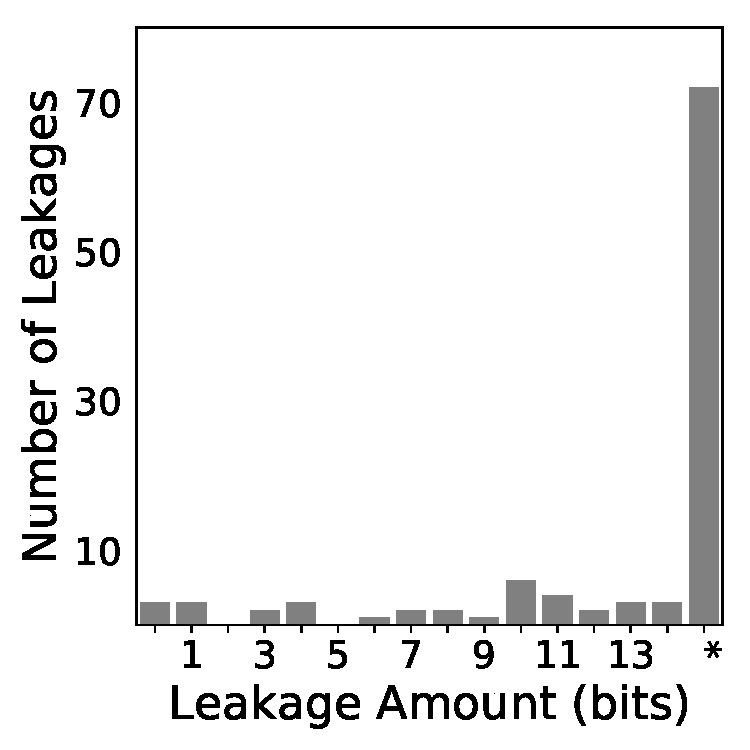
\includegraphics[width=.16\linewidth]{./figures/result/RSA-openssl-0-9-7.pdf}
        \label{fig:rsa-1}
    }
    \subfloat[OpenSSL 1.0.2f]{
        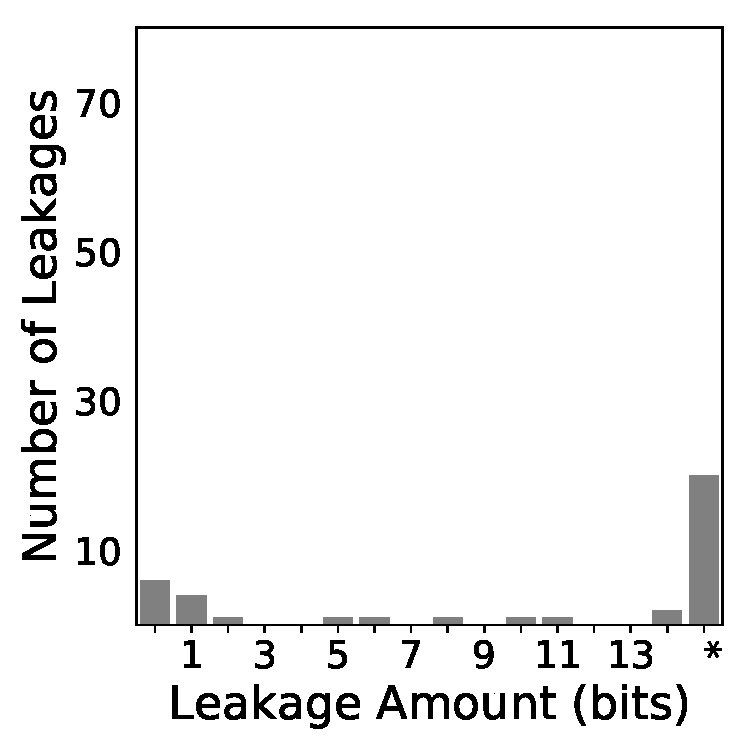
\includegraphics[width=.16\linewidth]{./figures/result/RSA-openssl-1-0-2f.pdf}
        \label{fig:rsa-2}
    }
    \subfloat[OpenSSL 1.0.2k]{
        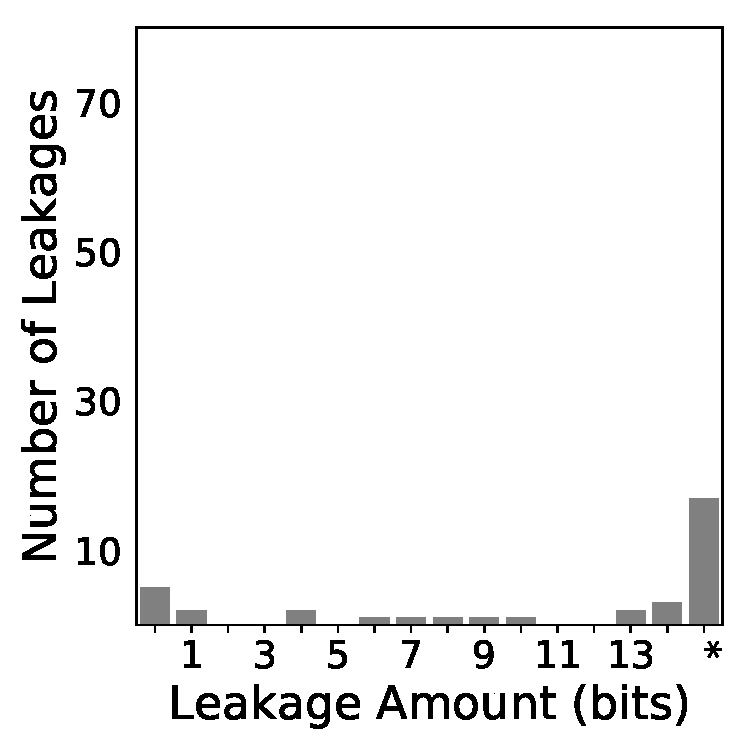
\includegraphics[width=.16\linewidth]{./figures/result/RSA-openssl-1-0-2k.pdf}
        \label{fig:rsa-3}
    }
    \subfloat[OpenSSL 1.1.0f]{
        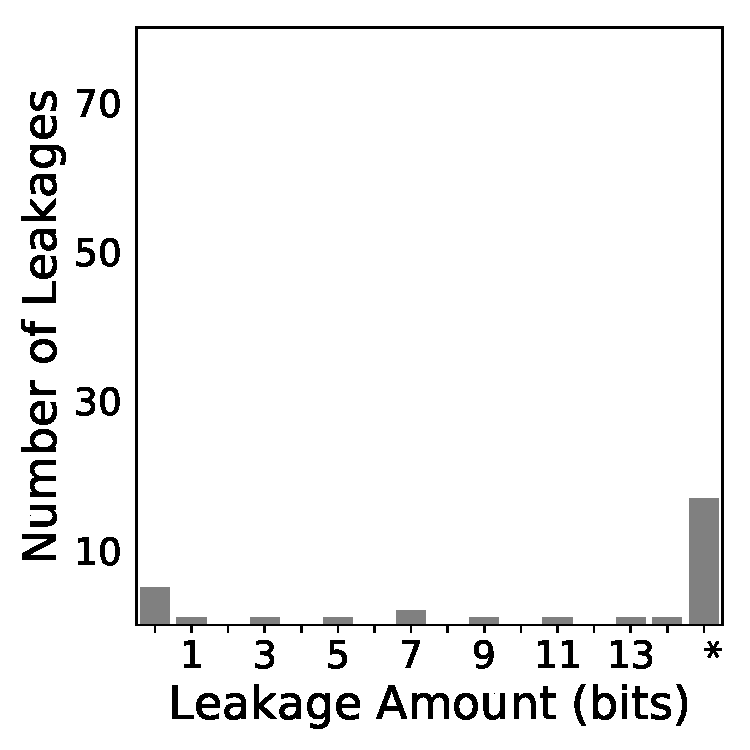
\includegraphics[width=.16\linewidth]{./figures/result/RSA-openssl-1-1-0f.pdf}
        \label{fig:rsa-4}
    }
    \subfloat[OpenSSL 1.1.1]{
        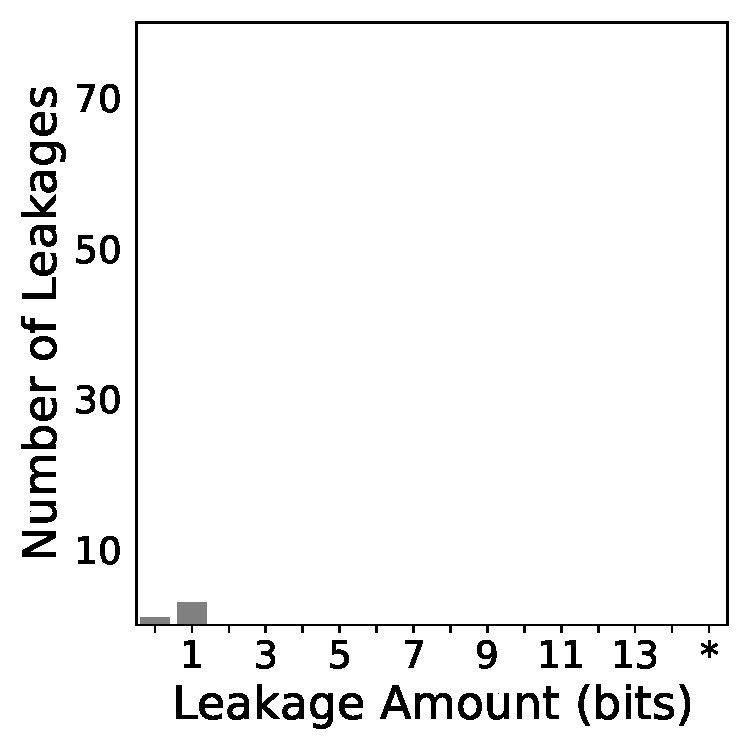
\includegraphics[width=.16\linewidth]{./figures/result/RSA-openssl-1-1-1.pdf}
        \label{fig:rsa-5}
    }
    \subfloat[OpenSSL 1.1.1g]{
        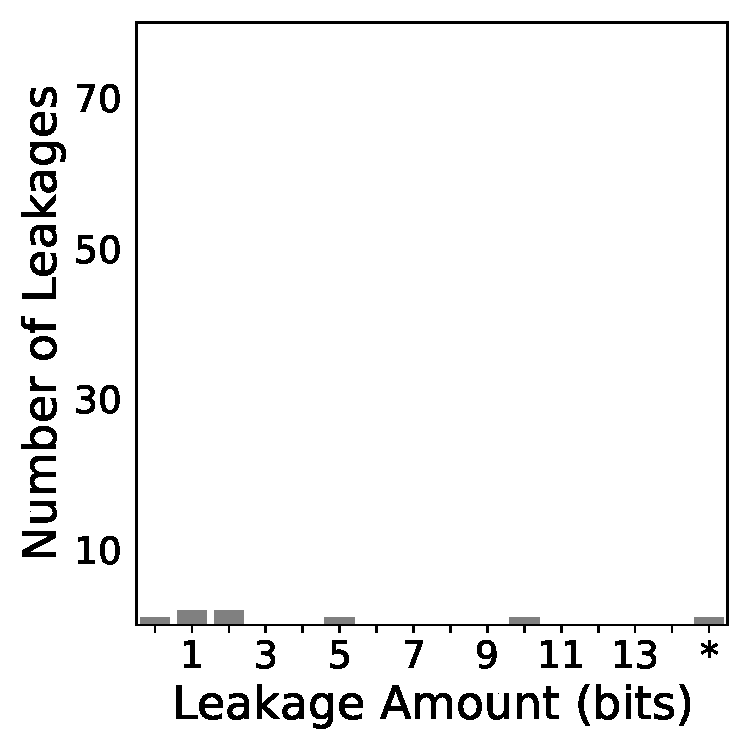
\includegraphics[width=.16\linewidth]{./figures/result/RSA-openssl-1-1-1g.pdf}
        \label{fig:rsa-6}
    }
    \caption{Side-channel leakages in different implementations of RSA in OpenSSL\@. 
        We round the number of leaked information into the nearest integer. 
        The mark $*$ means timeout (see \S\ref{loc:timeout}).}
    \label{fig:rsa}
    \vspace*{-20pt}
\end{figure*}
We also evaluate \tool{} on RSA. Due to the page limit,
we do not present the detailed leakage report. %, which is available online at the tool release website.
%% \jl{where?}. In general,
%% developers are interested in fixing side-channel vulnerabilities for the RSA implementations.
%% \jl{Then maybe find some space to present these results?}
 As shown in Figure~\ref{fig:rsa}, the result indicates that the newer
versions of OpenSSL leak less information than earlier
versions. After version 0.9.7g, OpenSSL adopts a fixed-window \textsf{mod\_exp\_mont}
implementation for RSA\@. With this design, the sequence of squares and
multiples and the memory access patterns are independent of the secret key.
\tool{}'s result confirms the new exponentiation implementation has mitigated 
most leakages effectively because the four newer versions have fewer
leakages than version 0.9.7, which introduced this change.
OpenSSL version 1.0.2f, 1.0.2k, and 1.1.0f almost have the
same amount of leakage. We check the ChangeLog and find only one change to
patch vulnerability CVE-2016-0702. 
\tool{} finds OpenSSL 1.1.1 and 1.1.1g have significantly less
leaked information than other versions.
We check the ChangeLog of these two versions and find a claim that
the new RSA implementation adopts ``numerous side-channel attack mitigation'', 
which proves the effectiveness of our quantifying method.
We also observe the latest version (1.1.1g) contains some new leakages. We have
contacted the developers and they have confirmed our findings.



Our quantification result shows vulnerabilities
that leak significant amounts of information
are more likely to be fixed in the updated version.
As presented in Figure~\ref{fig:rsa}, 
OpenSSL 0.9.7 has several severe leaks from
function \textsf{bn\_sqr\_comba8}, which is a main 
component of the OpenSSL big number implementation.
Shown in Figure~\ref{fig:old_sqr2}, it has a 
secret-dependent control flow at line 8.
The value of the function parameter \textbf{a} is derived from
the secret key. 
As function \textsf{bn\_sqr\_comba8}
calls the macro (\textsf{sqr\_add\_c2}) multiple times, 
and the code can leak some information each time.
\tool{} indicates the vulnerability is quite serious. 
It was patched in OpenSSL 1.1.1\@. In 
Figure~\ref{fig:new_sqr2}, control-flows transfers are replaced
so there are no leaks in the function
\textsf{sqr\_add\_c2} in OpenSSL 1.1.1\@. We note
that line 4 and 9 in Figure~\ref{fig:old_sqr2} both contain if branches.
However, they are not leaks because
most compilers use \emph{add with carry} instruction to eliminate the branch.
In addition, branches can be compiled into non-branch machine instructions 
with conditional moves. 
We notice a bitwise operation in Libgcrypt 1.8.5 is compiled to a conditional 
jump, which leads to a side-channel leakage.
Therefore, source-level code reviews are not accurate
enough to detect side-channels. 

For vulnerabilities that leak less information,
developers are more reluctant to fix them. 
For example, OpenSSL 0.9.7 adopts a fixed windows version of 
function \textsf{BN\_mod\_exp\_mont\_consttime} to replace original function
\textsf{BN\_mod\_exp\_mont}.
\tool{} detects a minor vulnerability in the original function that can
leak the last bit of the big number \textbf{m}. In the updated version,
developers make the fixed windows the default option and rewrite most of the 
function. However, the leakage site still exists in OpenSSL 1.1.1.
\begin{figure}
    \centering
    \begin{lstlisting}[xleftmargin=.02\textwidth,xrightmargin=.01\textwidth]
# define mul_add_c2(a,b,c0,c1,c2)                    \
    t=(BN_ULLONG)a*b;                                \
    tt=(t+t)&BN_MASK;                                \
    if (tt < t) c2++;                                \
    t1=(BN_ULONG)Lw(tt);                             \
    t2=(BN_ULONG)Hw(tt);                             \
    c0=(c0+t1)&BN_MASK2;                             \
    if ((c0 < t1) && (((++t2)&BN_MASK2) == 0)) c2++; \
    c1=(c1+t2)&BN_MASK2; if ((c1) < t2) c2++;
\end{lstlisting}
    \vspace*{-6pt}
    \caption{Macro \textsf{sqr\_add\_c2} in OpenSSL 0.9.7}
    \label{fig:old_sqr2}
    \vspace*{-8pt}
\end{figure}


\begin{figure}
    \centering
    \begin{lstlisting}[xleftmargin=.02\textwidth,xrightmargin=.01\textwidth]
# define mul_add_c2(a,b,c0,c1,c2)      do { \
    BN_ULONG ta = (a), tb = (b);            \
    BN_ULONG lo, hi, tt;                    \
    BN_UMULT_LOHI(lo,hi,ta,tb);             \
    c0 += lo; tt = hi+((c0<lo)?1:0);        \
    c1 += tt; c2 += (c1<tt)?1:0;            \
    c0 += lo; hi += (c0<lo)?1:0;            \
    c1 += hi; c2 += (c1<hi)?1:0;            \
    } while(0)
\end{lstlisting}
    \vspace*{-6pt}
    \caption{Macro \textsf{sqr\_add\_c2} in OpenSSL 1.1.1}
    \label{fig:new_sqr2}
    \vspace*{-10pt}
\end{figure}


\subsubsection{Monocypher}\label{eval:mono}
Monocypher is a small, easy to use cryptographic library with
performance comparable to LibSodium~\cite{libsodium} and NaCl~\cite{bernstein2012security}. 
We choose four ciphers that are 
designed to be side-channel resistant from the library.
Because those ciphers have no 
data flow from secrets to branch conditions and load addresses.
Monocypher should be safe under our threat models. 
We analyze those ciphers with \tool{}, and it reports no leaks.
This indicates that \tool{} is effective for validating countermeasures.
